Consider the following BVP with inhomogeneous boundary conditions conditions:
\begin{eqnarray*}
 -((1+x^2)u')'&=&x, \ 0<x<1, \\
u(0)&=&1, \\
u(1)&=&2. \\
\end{eqnarray*}

\begin{enumerate}
%\item Determine the exact solution to the above differential equation.
\item Let $x_0 = 0, x_1, \ldots, x_N, x_{N+1} = 1$ be a grid of points where $x_i = ih$.  Compute the finite element solution of this BVP using piecewise linear basis functions
\[
\phi_i(x) = \left\{
\begin{array}{ll}
\displaystyle{{x-x_{i-1}\over h}} & \mbox{if }x\in [x_{i-1}, x_i);\\
\displaystyle{{x_{i+1}-x\over h}} & \mbox{if }x\in [x_i, x_{i+1});\\
0 & \mbox{otherwise};
\end{array}\right.
\]
Plot the Galerkin solutions with $N=4, 8, 16, 32$ superimposed on each other.  \emph{You may wish to start with the codes from HW 8.}
\item In general, inhomogeneous boundary conditions are treated by decomposing $u(x)$ into 
\[
u(x) = w(x) + g(x)
\]
where $w(0) = w(1) = 0$ and $g(x)$ is any function satisfying inhomogeneous boundary conditions (this is referred to as the \emph{lift}).  We should make sure that the finite element solution does not depend on what lift we choose.  

Let $g(x) = 1 + x$; compute what modifications must be made to the load vector in order to compute the solution in this case.  
\item Using the above modifications for $g(x) = 1+x$, plot in \textsc{Matlab} the solution $u_N(x)$ for $N = 4,8,16,32$.  Verify that these solutions should look identical to the solutions from (a).  
\end{enumerate}

%%%%%%%%%%%%%%%%%%%%%%%%%%%%%%%%%%%%%%%%%%%%%%%%%%%%%%%%%%%%%%%%%%%%%%%%%%%%%%%%

\ifthenelse{\boolean{showsols}}{
\begin{solution}
\begin{enumerate}
\item In class, we showed that the resulting finite element system $K\alpha = b$ satisfied 
\[
K_{ij} = a(\phi_j,\phi_i), \quad b_i = \begin{cases}
(f,\phi_1) - u(0)a(\phi_{0},\phi_1) & i = 1\\
(f,\phi_i) & 1<i<N \\
(f,\phi_N) - u(1)a(\phi_{N+1},\phi_N) & i = N.
\end{cases}
\]
In Homework 8, we computed $K_{ij}$, so here we will focus only on computing $b_i$.  

Since $a(u,v) = \int_0^1(1+x^2) \pd{u}{x}{}\pd{v}{x}{}$, and $\phi_0$ is piecewise linear and nonzero only on the interval $[x_0, x_1] = [0,h]$,
\[
a(\phi_0,\phi_1) = \int_0^h (1+x^2)\frac{-1}{h^2} = \frac{1}{h^2} \left[x + \frac{x^3}{3}\right]_0^h = \frac{1}{h} + \frac{h}{3}.
\]
Similarly, $\phi_{N+1}$ is nonzero only on $[x_N,x_{N+1}] = [1-h,h]$, which gives
\[
a(\phi_{N+1},\phi_N) = \int_{1-h}^1 (1+x^2)\frac{-1}{h^2} = \frac{1}{h^2} \left[x + \frac{x^3}{3}\right]_{1-h}^1 = \frac{2h}{3} + \frac{4}{h} - 2.
\]
Then, since $a(\phi_0,\phi_1)$ and $a(\phi_{N+1},\phi_N)$ are now given, we can compute $b_i$ using the above formula.  

The graph produced by the finite element solution for $N = 4,8,16, 32$ is shown below
\begin{figure}
\centering
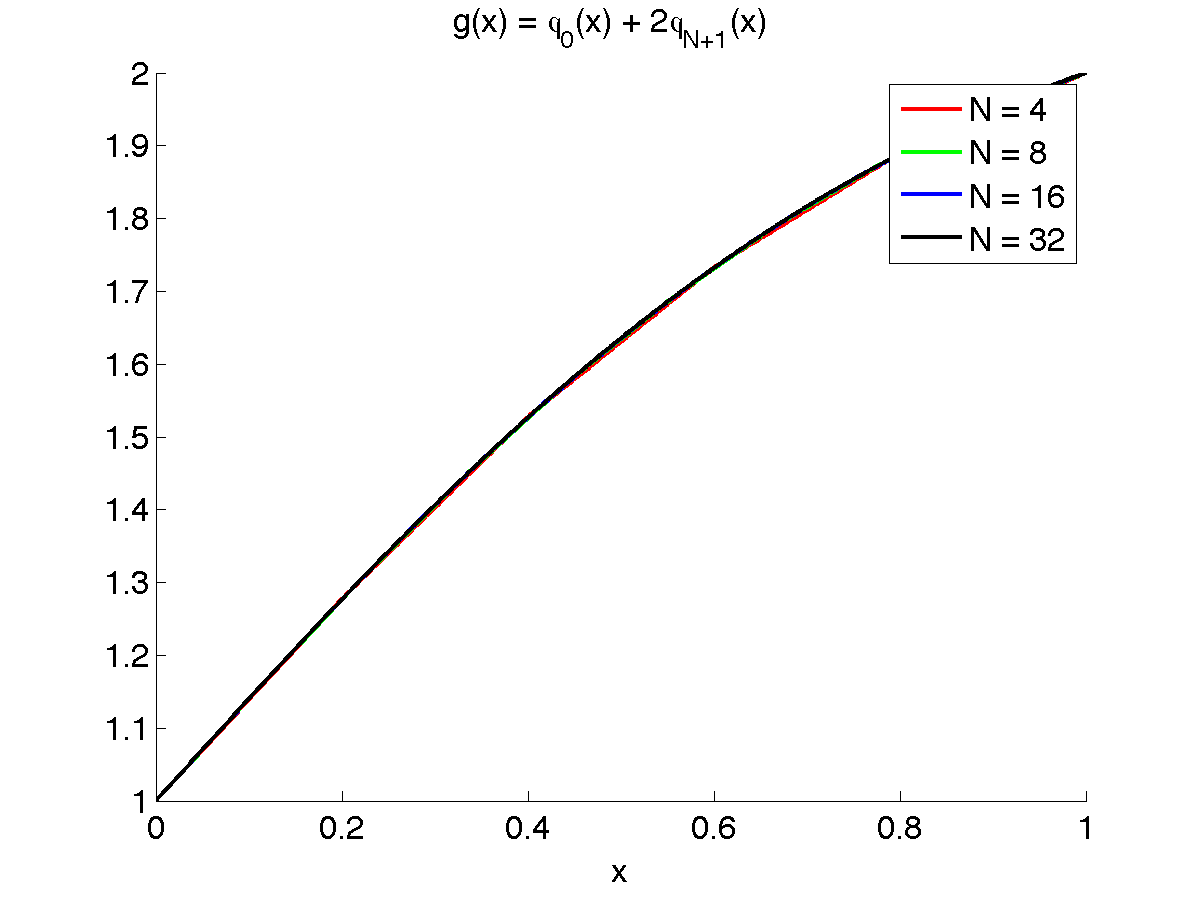
\includegraphics[width = .4\textwidth]{p1a.png}
\end{figure}

\item By changing $g(x)$ to $1+x$ and having $u(x) = w(x) + g(x)$, the more general form of the finite element equation needs to hold: 
\[
a(w,\phi_i) = (f,\phi_i) - a(g,\phi_i), \quad i = 1,\ldots, N.
\]
Then, since $\pd{g}{x}{} = 1$, we can write
\[
a(g,\phi_i) = \int_0^1 (1+x^2) \pd{\phi_i}{x}{} = \frac{1}{h} \left(\int_{x_{i-1}}^{x_i} (1+x^2) - \int_{x_{i}}^{x_{i+1}} (1+x^2)\right)   
\]
Plugging in $x_i = ih$ reduces the above to $a(g,\phi_i) = -2 i h^2$.  


Another alternative way to solve this problem is to notice that you can represent $g(x)$ exactly using a linear combination of $\phi_0,\ldots, \phi_{N+1}$
\[
g(x) = \sum_{j=0}^{N+1} g(x_j)\phi_j(x).
\]
You can then use the fact that
\begin{align*}
a(g,\phi_i) &= \sum_{j=1}^N g(x_j)a(\phi_j,\phi_i) + g(0) a(\phi_0,\phi_i) + g(1) a(\phi_{N+1},\phi_N)\\
 &= \sum_{j=1}^N g(x_j) K_{ij} + a(\phi_0,\phi_i) + 2 a(\phi_{N+1},\phi_N),
\end{align*}
which reduces down to using $K_{ij}$ (from Hw 8) and the solution from part (a) for $a(\phi_0,\phi_i)$ and $a(\phi_{N+1},\phi_i)$, which are zero unless $i = 1$ or $i = N$.  
\item The figure produced using $g(x) = 1+ x$ is as follow:
\begin{figure}
\centering
\subfigure[$g(x) = \phi_0(x) + 2\phi_{N+1}(x)$]{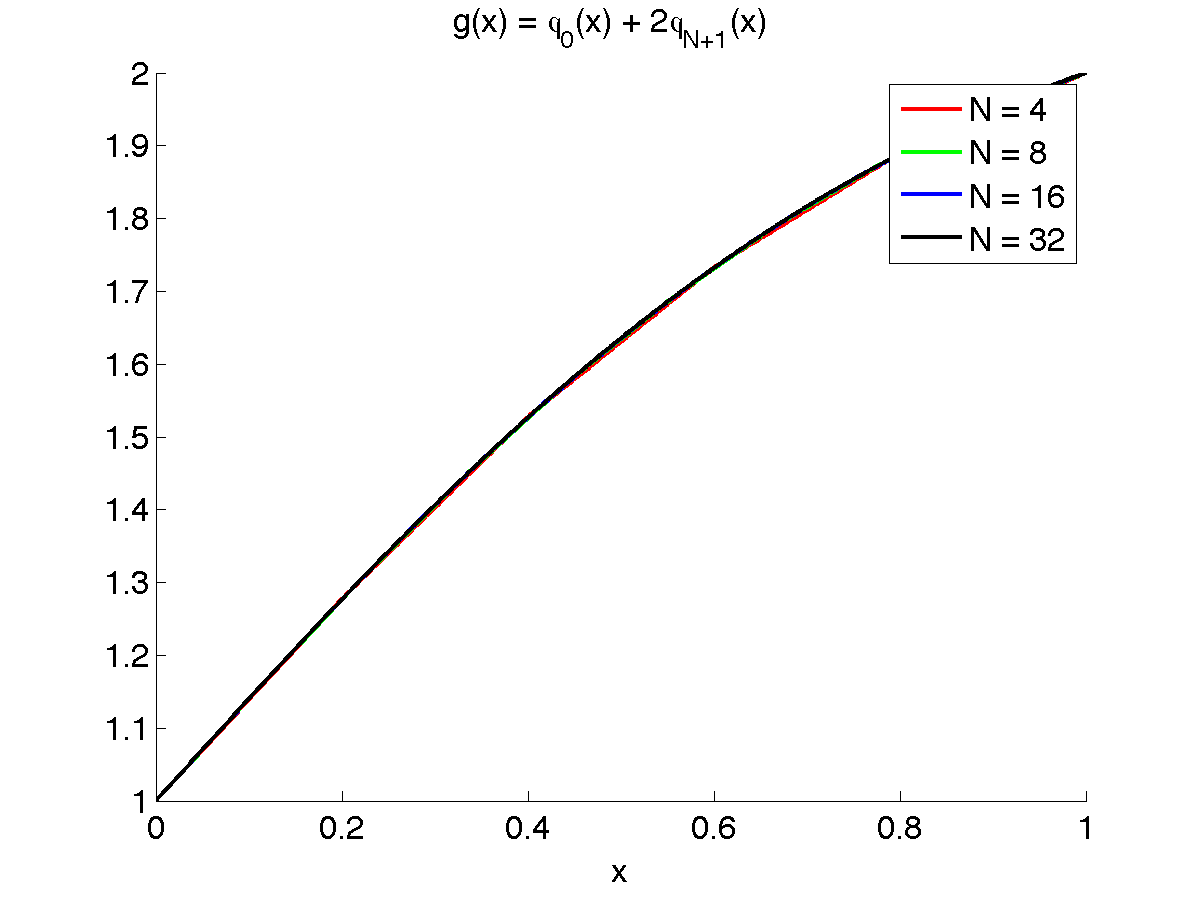
\includegraphics[width = .4\textwidth]{p1a.png}}
\subfigure[$g(x) = 1+x$]{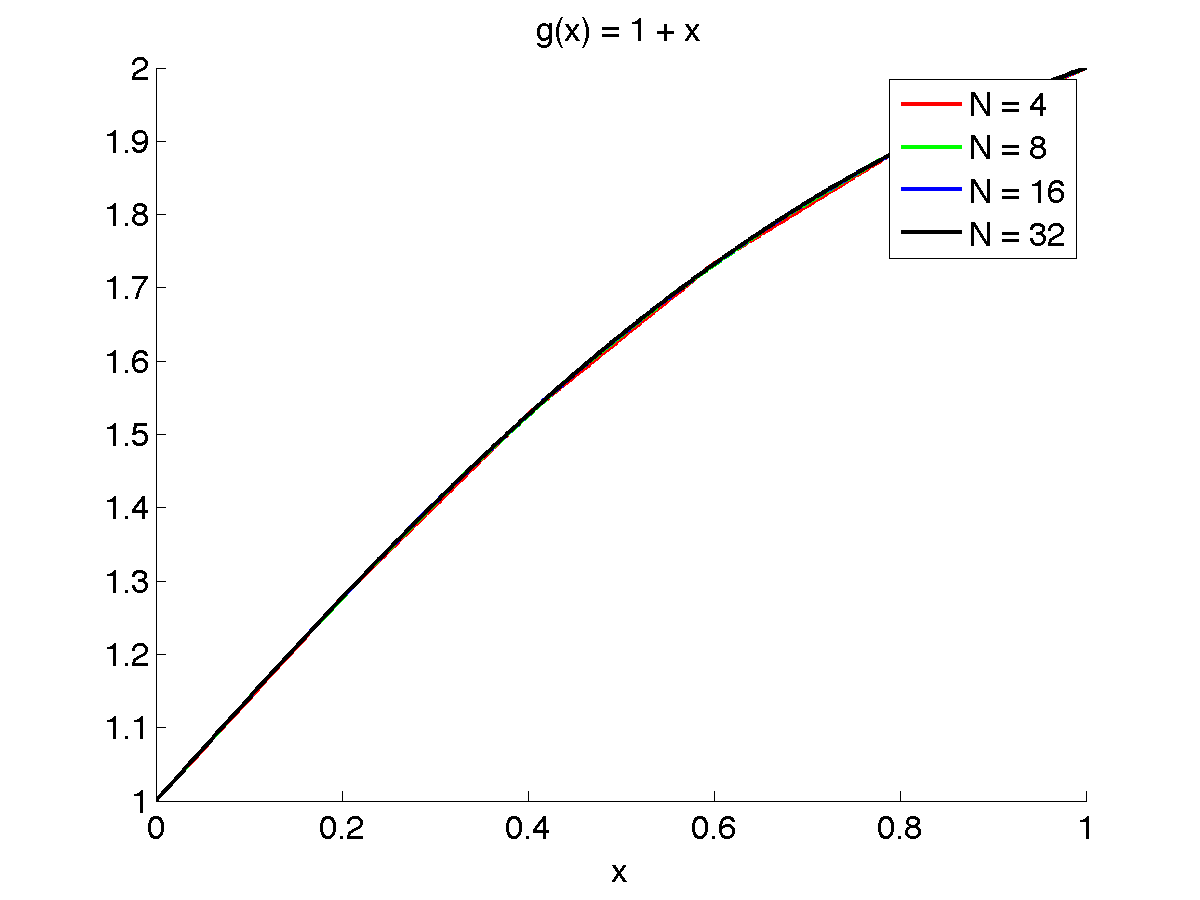
\includegraphics[width = .4\textwidth]{p1c.png}}
\end{figure}
\end{enumerate}

The code to compute both part (a) and (c) is below as well.  
\input inhbc_code
\end{solution}
}{}

